\documentclass[twoside,11pt]{article}

% ? Specify used packages
\usepackage{graphicx}        %  Use this one for final production.
% \usepackage[draft]{graphicx} %  Use this one for drafting.
% ? End of specify used packages

\pagestyle{myheadings}

% -----------------------------------------------------------------------------
% ? Document identification
% Fixed part
\newcommand{\stardoccategory}  {Starlink User Note}
\newcommand{\stardocinitials}  {SUN}
\newcommand{\stardocsource}    {sun\stardocnumber}

% Variable part - replace [xxx] as appropriate.
\newcommand{\stardocnumber}    {226.8}
\newcommand{\stardocauthors}   {A.J. Chipperfield\\
                                P.W. Draper}
\newcommand{\stardocdate}      {24th April 2004}
\newcommand{\stardoctitle}     {EXTRACTOR\\
                                An Astronomical Source Detection Program}
\newcommand{\stardocmanual}    {User Manual}
\newcommand{\stardocabstract}  {\EXTRACTOR\ will detect sources in
an astronomical image and build a catalogue listing them. It is based on the
popular \SExtractor\ program, has very flexible configuration
facilities and can handle images and catalogues in a variety of formats.}
% ? End of document identification

\newcommand{\sexversion}{2.3.2}

% -----------------------------------------------------------------------------

% +
%  Name:
%     sun.tex
%
%  Purpose:
%     Template for Starlink User Note (SUN) documents.
%     Refer to SUN/199
%
%  Authors:
%     AJC: A.J.Chipperfield (Starlink, RAL)
%     BLY: M.J.Bly (Starlink, RAL)
%     PWD: Peter W. Draper (Starlink, Durham University)
%
%  History:
%     17-JAN-1996 (AJC):
%        Original with hypertext macros, based on MDL plain originals.
%     16-JUN-1997 (BLY):
%        Adapted for LaTeX2e.
%        Added picture commands.
%     13-AUG-1998 (PWD):
%        Converted for use with LaTeX2HTML version 98.2 and
%        Star2HTML version 1.3.
%     {Add further history here}
%
% -

\newcommand{\stardocname}{\stardocinitials /\stardocnumber}
\markboth{\stardocname}{\stardocname}
\setlength{\textwidth}{160mm}
\setlength{\textheight}{230mm}
\setlength{\topmargin}{-2mm}
\setlength{\oddsidemargin}{0mm}
\setlength{\evensidemargin}{0mm}
\setlength{\parindent}{0mm}
\setlength{\parskip}{\medskipamount}
\setlength{\unitlength}{1mm}

% -----------------------------------------------------------------------------
%  Hypertext definitions.
%  ======================
%  These are used by the LaTeX2HTML translator in conjunction with star2html.

%  Comment.sty: version 2.0, 19 June 1992
%  Selectively in/exclude pieces of text.
%
%  Author
%    Victor Eijkhout                                      <eijkhout@cs.utk.edu>
%    Department of Computer Science
%    University Tennessee at Knoxville
%    104 Ayres Hall
%    Knoxville, TN 37996
%    USA

%  Do not remove the %begin{latexonly} and %end{latexonly} lines (used by
%  LaTeX2HTML to signify text it shouldn't process).
%begin{latexonly}
\makeatletter
\def\makeinnocent#1{\catcode`#1=12 }
\def\csarg#1#2{\expandafter#1\csname#2\endcsname}

\def\ThrowAwayComment#1{\begingroup
    \def\CurrentComment{#1}%
    \let\do\makeinnocent \dospecials
    \makeinnocent\^^L% and whatever other special cases
    \endlinechar`\^^M \catcode`\^^M=12 \xComment}
{\catcode`\^^M=12 \endlinechar=-1 %
 \gdef\xComment#1^^M{\def\test{#1}
      \csarg\ifx{PlainEnd\CurrentComment Test}\test
          \let\html@next\endgroup
      \else \csarg\ifx{LaLaEnd\CurrentComment Test}\test
            \edef\html@next{\endgroup\noexpand\end{\CurrentComment}}
      \else \let\html@next\xComment
      \fi \fi \html@next}
}
\makeatother

\def\includecomment
 #1{\expandafter\def\csname#1\endcsname{}%
    \expandafter\def\csname end#1\endcsname{}}
\def\excludecomment
 #1{\expandafter\def\csname#1\endcsname{\ThrowAwayComment{#1}}%
    {\escapechar=-1\relax
     \csarg\xdef{PlainEnd#1Test}{\string\\end#1}%
     \csarg\xdef{LaLaEnd#1Test}{\string\\end\string\{#1\string\}}%
    }}

%  Define environments that ignore their contents.
\excludecomment{comment}
\excludecomment{rawhtml}
\excludecomment{htmlonly}

%  Hypertext commands etc. This is a condensed version of the html.sty
%  file supplied with LaTeX2HTML by: Nikos Drakos <nikos@cbl.leeds.ac.uk> &
%  Jelle van Zeijl <jvzeijl@isou17.estec.esa.nl>. The LaTeX2HTML documentation
%  should be consulted about all commands (and the environments defined above)
%  except \xref and \xlabel which are Starlink specific.

\newcommand{\htmladdnormallinkfoot}[2]{#1\footnote{#2}}
\newcommand{\htmladdnormallink}[2]{#1}
\newcommand{\htmladdimg}[1]{}
\newcommand{\hyperref}[4]{#2\ref{#4}#3}
\newcommand{\htmlref}[2]{#1}
\newcommand{\htmlimage}[1]{}
\newcommand{\htmladdtonavigation}[1]{}

\newenvironment{latexonly}{}{}
\newcommand{\latex}[1]{#1}
\newcommand{\html}[1]{}
\newcommand{\latexhtml}[2]{#1}
\newcommand{\HTMLcode}[2][]{}

%  Starlink cross-references and labels.
\newcommand{\xref}[3]{#1}
\newcommand{\xlabel}[1]{}

%  LaTeX2HTML symbol.
\newcommand{\latextohtml}{\LaTeX2\texttt{HTML}}

%  Define command to re-centre underscore for Latex and leave as normal
%  for HTML (severe problems with \_ in tabbing environments and \_\_
%  generally otherwise).
\renewcommand{\_}{\texttt{\symbol{95}}}

% -----------------------------------------------------------------------------
%  Debugging.
%  =========
%  Remove % on the following to debug links in the HTML version using Latex.

% \newcommand{\hotlink}[2]{\fbox{\begin{tabular}[t]{@{}c@{}}#1\\\hline{\footnotesize #2}\end{tabular}}}
% \renewcommand{\htmladdnormallinkfoot}[2]{\hotlink{#1}{#2}}
% \renewcommand{\htmladdnormallink}[2]{\hotlink{#1}{#2}}
% \renewcommand{\hyperref}[4]{\hotlink{#1}{\S\ref{#4}}}
% \renewcommand{\htmlref}[2]{\hotlink{#1}{\S\ref{#2}}}
% \renewcommand{\xref}[3]{\hotlink{#1}{#2 -- #3}}
%end{latexonly}
% -----------------------------------------------------------------------------
% ? Document specific \newcommand or \newenvironment commands.
\newcommand{\EXTRACTOR}{\texttt{EXTRACTOR}}
\newcommand{\CONVERT}{\texttt{CONVERT}}
\newcommand{\SExtractor}{\texttt{SExtractor}}
\newcommand{\SExtractorURL}{http://terapix.iap.fr/soft/sextractor}
\newcommand{\DUMMIESURL}{http://www-int.stsci.edu/~holwerda/se.html}
\newcommand{\IRAFURL}{http://www.starlink.rl.ac.uk/iraf/web/iraf-homepage.html}
\newcommand{\FITSURL}{http://fits.gsfc.nasa.gov/}
\newcommand{\nMUD}{mud165.ps}
\newcommand{\dash}{--}
\begin{htmlonly}
  \newcommand{\dash}{-}
\end{htmlonly}
%+
%  Name:
%     SST.TEX

%  Purpose:
%     Define LaTeX commands for laying out Starlink routine descriptions.

%  Language:
%     LaTeX

%  Type of Module:
%     LaTeX data file.

%  Description:
%     This file defines LaTeX commands which allow routine documentation
%     produced by the SST application PROLAT to be processed by LaTeX and
%     by LaTeX2html. The contents of this file should be included in the
%     source prior to any statements that make of the sst commnds.

%  Notes:
%     The style file html.sty provided with LaTeX2html needs to be used.
%     This must be before this file.

%  Authors:
%     RFWS: R.F. Warren-Smith (STARLINK)
%     PDRAPER: P.W. Draper (Starlink - Durham University)

%  History:
%     10-SEP-1990 (RFWS):
%        Original version.
%     10-SEP-1990 (RFWS):
%        Added the implementation status section.
%     12-SEP-1990 (RFWS):
%        Added support for the usage section and adjusted various spacings.
%     8-DEC-1994 (PDRAPER):
%        Added support for simplified formatting using LaTeX2html.
%     {enter_further_changes_here}

%  Bugs:
%     {note_any_bugs_here}

%-

%  Define length variables.
\newlength{\sstbannerlength}
\newlength{\sstcaptionlength}
\newlength{\sstexampleslength}
\newlength{\sstexampleswidth}

%  Define a \tt font of the required size.
\latex{\newfont{\ssttt}{cmtt10 scaled 1095}}
\html{\newcommand{\ssttt}{\tt}}

%  Define a command to produce a routine header, including its name,
%  a purpose description and the rest of the routine's documentation.
\newcommand{\sstroutine}[3]{
   \goodbreak
   \rule{\textwidth}{0.5mm}
   \vspace{-7ex}
   \newline
   \settowidth{\sstbannerlength}{{\Large {\bf #1}}}
   \setlength{\sstcaptionlength}{\textwidth}
   \setlength{\sstexampleslength}{\textwidth}
   \addtolength{\sstbannerlength}{0.5em}
   \addtolength{\sstcaptionlength}{-2.0\sstbannerlength}
   \addtolength{\sstcaptionlength}{-5.0pt}
   \settowidth{\sstexampleswidth}{{\bf Examples:}}
   \addtolength{\sstexampleslength}{-\sstexampleswidth}
   \parbox[t]{\sstbannerlength}{\flushleft{\Large {\bf #1}}}
   \parbox[t]{\sstcaptionlength}{\center{\Large #2}}
   \parbox[t]{\sstbannerlength}{\flushright{\Large {\bf #1}}}
   \begin{description}
      #3
   \end{description}
}

%  Format the description section.
\newcommand{\sstdescription}[1]{\item[Description:] #1}

%  Format the usage section.
\newcommand{\sstusage}[1]{\item[Usage:] \mbox{}
\\[1.3ex]{\raggedright \ssttt #1}}

%  Format the invocation section.
\newcommand{\sstinvocation}[1]{\item[Invocation:]\hspace{0.4em}{\tt #1}}

%  Format the arguments section.
\newcommand{\sstarguments}[1]{
   \item[Arguments:] \mbox{} \\
   \vspace{-3.5ex}
   \begin{description}
      #1
   \end{description}
}

%  Format the returned value section (for a function).
\newcommand{\sstreturnedvalue}[1]{
   \item[Returned Value:] \mbox{} \\
   \vspace{-3.5ex}
   \begin{description}
      #1
   \end{description}
}

%  Format the parameters section (for an application).
\newcommand{\sstparameters}[1]{
   \item[Parameters:] \mbox{} \\
   \vspace{-3.5ex}
   \begin{description}
      #1
   \end{description}
}

%  Format the examples section.
\newcommand{\sstexamples}[1]{
   \item[Examples:] \mbox{} \\
   \vspace{-3.5ex}
   \begin{description}
      #1
   \end{description}
}

%  Define the format of a subsection in a normal section.
\newcommand{\sstsubsection}[1]{ \item[{#1}] \mbox{} \\}

%  Define the format of a subsection in the examples section.
\newcommand{\sstexamplesubsection}[2]{\sloppy
\item[\parbox{\sstexampleslength}{\ssttt #1}] \mbox{} \vspace{1.0ex}
\\ #2 }

%  Format the notes section.
\newcommand{\sstnotes}[1]{\item[Notes:] \mbox{} \\[1.3ex] #1}

%  Provide a general-purpose format for additional (DIY) sections.
\newcommand{\sstdiytopic}[2]{\item[{\hspace{-0.35em}#1\hspace{-0.35em}:}]
\mbox{} \\[1.3ex] #2}

%  Format the implementation status section.
\newcommand{\sstimplementationstatus}[1]{
   \item[{Implementation Status:}] \mbox{} \\[1.3ex] #1}

%  Format the bugs section.
\newcommand{\sstbugs}[1]{\item[Bugs:] #1}

%  Format a list of items while in paragraph mode.
\newcommand{\sstitemlist}[1]{
  \mbox{} \\
  \vspace{-3.5ex}
  \begin{itemize}
     #1
  \end{itemize}
}

%  Define the format of an item.
\newcommand{\sstitem}{\item}

%% Now define html equivalents of those already set. These are used by
%  latex2html and are defined in the html.sty files.
\begin{htmlonly}

%  sstroutine.
   \newcommand{\sstroutine}[3]{
      \subsection{#1\xlabel{#1}-\label{#1}#2}
      \begin{description}
         #3
      \end{description}
   }

%  sstdescription
   \newcommand{\sstdescription}[1]{\item[Description:]
      \begin{description}
         #1
      \end{description}
      \\
   }

%  sstusage
   \newcommand{\sstusage}[1]{\item[Usage:]
      \begin{description}
         {\ssttt #1}
      \end{description}
      \\
   }

%  sstinvocation
   \newcommand{\sstinvocation}[1]{\item[Invocation:]
      \begin{description}
         {\ssttt #1}
      \end{description}
      \\
   }

%  sstarguments
   \newcommand{\sstarguments}[1]{
      \item[Arguments:] \\
      \begin{description}
         #1
      \end{description}
      \\
   }

%  sstreturnedvalue
   \newcommand{\sstreturnedvalue}[1]{
      \item[Returned Value:] \\
      \begin{description}
         #1
      \end{description}
      \\
   }

%  sstparameters
   \newcommand{\sstparameters}[1]{
      \item[Parameters:] \\
      \begin{description}
         #1
      \end{description}
      \\
   }

%  sstexamples
   \newcommand{\sstexamples}[1]{
      \item[Examples:] \\
      \begin{description}
         #1
      \end{description}
      \\
   }

%  sstsubsection
   \newcommand{\sstsubsection}[1]{\item[{#1}]}

%  sstexamplesubsection
   \newcommand{\sstexamplesubsection}[2]{\item[{\ssttt #1}] #2}

%  sstnotes
   \newcommand{\sstnotes}[1]{\item[Notes:] #1 }

%  sstdiytopic
   \newcommand{\sstdiytopic}[2]{\item[{#1}] #2 }

%  sstimplementationstatus
   \newcommand{\sstimplementationstatus}[1]{
      \item[Implementation Status:] #1
   }

%  sstitemlist
   \newcommand{\sstitemlist}[1]{
      \begin{itemize}
         #1
      \end{itemize}
      \\
   }
%  sstitem
   \newcommand{\sstitem}{\item}

\end{htmlonly}

%  End of "sst.tex" layout definitions.
%.

% ? End of document specific commands
% -----------------------------------------------------------------------------
%  Title Page.
%  ===========
\renewcommand{\thepage}{\roman{page}}
\begin{document}
\thispagestyle{empty}

%  Latex document header.
%  ======================
\begin{latexonly}
   CCLRC / \textsc{Rutherford Appleton Laboratory} \hfill \textbf{\stardocname}\\
   {\large Particle Physics \& Astronomy Research Council}\\
   {\large Starlink Project\\}
   {\large \stardoccategory\ \stardocnumber}
   \begin{flushright}
   \stardocauthors\\
   \stardocdate
   \end{flushright}
   \vspace{-4mm}
   \rule{\textwidth}{0.5mm}
   \vspace{4mm}
   \begin{center}
   {\LARGE\textbf{\stardoctitle} \\ [2.5ex]}
   \vspace{4mm}

% ? Add picture here if required for the LaTeX version.
   \includegraphics[scale=0.6]{sun226fig.ps}
% ? End of picture
   \end{center}

% ? Heading for abstract if used.
   \vspace{5mm}
   \begin{center}
      {\Large\textbf{Abstract}}
   \end{center}
% ? End of heading for abstract.
\end{latexonly}

%  HTML documentation header.
%  ==========================
\begin{htmlonly}
   \xlabel{}
   \begin{rawhtml} <H1 ALIGN=CENTER> \end{rawhtml}
      \stardoctitle
   \begin{rawhtml} </H1> <HR> \end{rawhtml}

% ? Add picture here if required for the hypertext version.
   \begin{center}
     \htmladdimg{sun226fig.gif}
   \end{center}
% ? End of picture

   \begin{rawhtml} <P> <I> \end{rawhtml}
   \stardoccategory\ \stardocnumber \\
   \stardocauthors \\
   \stardocdate
   \begin{rawhtml} </I> </P> <H3> \end{rawhtml}
      \htmladdnormallink{CCLRC / Rutherford Appleton Laboratory}
                        {http://www.cclrc.ac.uk}\\
      \htmladdnormallink{Particle Physics \& Astronomy Research Council}
                        {http://www.pparc.ac.uk} \\
   \begin{rawhtml} </H3> <H2> \end{rawhtml}
      \htmladdnormallink{Starlink Project}{http://www.starlink.ac.uk/}
   \begin{rawhtml} </H2> \end{rawhtml}
   \htmladdnormallink{\htmladdimg{source.gif} Retrieve hardcopy}
      {http://www.starlink.ac.uk/cgi-bin/hcserver?\stardocsource}\\

%  HTML document table of contents.
%  ================================
%  Add table of contents header and a navigation button to return to this
%  point in the document (this should always go before the abstract \section).
  \label{stardoccontents}
  \begin{rawhtml}
    <HR>
    <H2>Contents</H2>
  \end{rawhtml}
  \htmladdtonavigation{\htmlref{\htmladdimg{contents_motif.gif}}
        {stardoccontents}}

% ? New section for abstract if used.
  \section{\xlabel{abstract}Abstract}
% ? End of new section for abstract
\end{htmlonly}

% -----------------------------------------------------------------------------
% ? Document Abstract. (if used)
%  ==================
\stardocabstract
% ? End of document abstract
% -----------------------------------------------------------------------------
% ? Latex document Table of Contents (if used).
%  ===========================================
  \newpage
  \begin{latexonly}
    \setlength{\parskip}{0mm}
    \tableofcontents
    \setlength{\parskip}{\medskipamount}
    \markboth{\stardocname}{\stardocname}
  \end{latexonly}
% ? End of Latex document table of contents
% -----------------------------------------------------------------------------
\cleardoublepage
\renewcommand{\thepage}{\arabic{page}}
\setcounter{page}{1}

% ? Main text
\section{\xlabel{introduction}Introduction}
\EXTRACTOR\ is a program for automatically detecting objects on an
astronomical image and building a catalogue of their properties. It is
particularly suited for the reduction of large scale galaxy-survey
data, but also performs well on other astronomical images.

\EXTRACTOR\ is basically Emmanuel Bertin's \SExtractor\
(Source-Extractor) program\footnote{BERTIN E. and ARNOUTS S., 1996,
A\&AS 117,393} re-packaged for use in the
\xref{Starlink Software Environment}{sg4}{} \latex{(see SG/4)}.
This means that it uses the Starlink parameter system, accepts images in
\xref{NDF}{sun33}{abstract} format \latex{(see SUN/33)} and uses the
\xref{AST}{sun210}{} library \latex{(SUN/210)} for astrometry.

Extending the program to use NDFs allows it to read and write other
image formats using the NDF library \xref{`on-the-fly' conversion
facility}{ssn20}{abstract} \latex{(see SSN/20)}.  Conversion to and
from many ``standard'' astronomical
\xref{formats}{sun55}{the_default_conversion_commands} are available
by using the \xref{\CONVERT}{sun55}{abstract} package \latex{(see
SUN/55)} -- these include \htmladdnormallink{FITS}{\FITSURL} and
\htmladdnormallink{IRAF}{\IRAFURL} OIF.

An slightly modified version of \SExtractor\ \sexversion\ is also
included in the distribution of \EXTRACTOR.
You can find details of \SExtractor's operation, and how to configure
it, in the \htmladdnormallink{\SExtractor\ User's Guide}{\MUD} (which is
issued as a Starlink Miscellaneous User Document, MUD 165\footnote{Note this
document is still in draft, consequently you should read this in
conjunction with the \htmladdnormallink{A\&AS paper}{sexpaper.ps}
and the \htmladdnormallink{earlier SExtractor user document}{sex1_doc.ps}.})
\dash\ you configure \EXTRACTOR\
in much the same way, although with
\htmlref{some restrictions}{implementation_notes}
\latex{(see Section~\ref{implementation_notes})}. The \SExtractor\ home page
-- \htmladdnormallink{\texttt{\SExtractorURL}}{\SExtractorURL} -- 
offers more information, such as a link to the 
\htmladdnormallink{\textit{SExtractor for Dummies}}{\DUMMIESURL}.

This document describes how to run \EXTRACTOR, and includes
\htmlref{instructions for running \SExtractor}{running_sextractor}
from the Starlink distribution.

\section{\xlabel{running_extractor}Running \EXTRACTOR}

Like any Starlink program \EXTRACTOR\ may be run from the
Unix shell or from a user-interface such as
\xref{ICL}{sg5}{abstract} \latex{(see SG/5)}.
A useful summary of the rich variety of methods of specifying parameter values
is given in \xref{SUN/95}{sun95}{se_param}. C-shell users should also
consult \xref{SC/4}{sc4}{}, the C-Shell CookBook.

The examples below assume you are running from the Unix shell but the commands
and parameters are exactly the same from ICL.

After normal Starlink startup, at the shell prompt, type:
\begin{quote} \begin{verbatim}
% extractorsetup
\end{verbatim} \end{quote}
to initialise the package and then:
\begin{quote} \begin{verbatim}
% extractor
\end{verbatim} \end{quote}
to run the program.  You will now be prompted for the values of parameters
CONFIG and IMAGE in turn:
\begin{quote} \begin{verbatim}
CONFIG - Configuration file /'$EXTRACTOR_DIR/config/default.sex'/ >
IMAGE - Input image /'image'/ >
\end{verbatim} \end{quote}
where CONFIG is the name of the `preferences' file and IMAGE is the name of
the image file to be processed.

Suggested values are given between \texttt{//} in the prompt.  You can
accept the suggested values by just typing \verb!<RETURN>!.  If you
accept the suggested values shown above, \EXTRACTOR\ will process the
NDF \texttt{"image"} using the installed default configuration
files to produce a catalogue named \texttt{test.cat} (this name is
specified in the preferences file).

CONFIG has a `default' value of
\texttt{\$EXTRACTOR\_DIR/config/default.sex}.  This file has some
\htmlref{sensible defaults}{defaults} \latex{(described in
Section~\ref{defaults})} but you will probably want to copy it to your
own directories and modify it to your taste (as you would for the
native \SExtractor\ program).  Similarly with the other configuration
files.  The environment variable \texttt{EXTRACTOR\_DIR} is defined to
point to the directory containing the \EXTRACTOR\ program and the
\texttt{config} directory.

You can also provide parameter values on the command line.
Either positionally,
\begin{quote} \begin{verbatim}
% extractor image $EXTRACTOR_DIR/config/default.sex
\end{verbatim} \end{quote}
or by keyword,
\begin{quote} \begin{verbatim}
% extractor config=$EXTRACTOR_DIR/config/default.sex
\end{verbatim} \end{quote}
(In this case, you would be prompted for IMAGE but not for CONFIG.)

The additional parameters KEYWORDS, NAME and VALUE allow
configuration parameters specified in the preferences file to be overridden
without editing the file. For example:
\begin{quote} \begin{verbatim}
% extractor keywords=true
NAME - Parameter name /!/ > catalog_name
VALUE - Parameter value /!/ > sky.cat
NAME - Parameter name /!/ > catalog_type
VALUE - Parameter value /!/ > ascii_skycat
NAME - Parameter name /!/ >
CONFIG - Configuration file /'$EXTRACTOR_DIR/config/default.sex'/ >
IMAGE - Input image /'image'/ >
\end{verbatim} \end{quote}
would change the name and type of the catalogue produced (for this
run only). The list of changes is terminated by replying with the NULL
response (\texttt{!}) to the prompt.
The
\htmladdnormallink{\SExtractor\ User's Guide}{\MUD}\latex{ (MUD/165)}
gives a full list of possible parameter names and values, but it is only
sensible to change a few in this way.

\subsection{Running \EXTRACTOR\ from scripts}
If you'd like to run \EXTRACTOR\ from a script, just say for instance
sampling different populations of objects at different thresholds, you
can do this using the NAME VALUE parameters (avoiding the need to have
multiple configuration files), but you need to adopt a slightly
different strategy to normal programs. Here's one example script:

\newpage
\begin{center}
\latexhtml{\fbox{\textbf{Example batch script}}}{\textbf{Example batch script}}
\end{center}
\begin{quote} \begin{verbatim}
#!/bin/csh

#  Initialize EXTRACTOR
extractorsetup

#  Extract all objects above 1 sigma
extractor keywords=true image=image config=default.sex <<EOF
catalog_name
thresh1.cat
detect_thresh
1.0
!
EOF

# Extract all objects above 2 sigma and measure on a different image.
extractor keywords image='"detect,measure"' config=default.sex <<EOF
catalog_name
thresh2.cat
detect_thresh
2.0
!
EOF
\end{verbatim} \end{quote}
Using the C-shell \verb+<<EOF+ mechanism allows you to send
information to the program as if you're typing it in.


\section{\xlabel{the_default_configuration}\label{defaults}\xlabel{defaults}The default configuration}

The directory \texttt{\$EXTRACTOR\_DIR/config} contains the default
configuration files.

The main `preferences' file, \texttt{default.sex} is listed in
Appendix~\ref{default_sex}.
You will see that it uses the default convolution mask and `Neural Network
Weights' file, and specifies that an ASCII\_HEAD-type catalogue named
\texttt{test.cat} is to be produced.

File \texttt{default.param} specifies which measurements are to be
made of the objects (these are all written to the output
catalogue). The defaults are:
\begin{quote}\begin{verbatim}
NUMBER
X_IMAGE
Y_IMAGE
FLUX_ISO
FLUXERR_ISO
FLUX_AUTO
FLUXERR_AUTO
FLUX_MAX
ISOAREA_IMAGE
CXX_IMAGE
CYY_IMAGE
CXY_IMAGE
THETA_IMAGE
ELLIPTICITY
FLAGS
\end{verbatim}\end{quote}

For a full description of the meaning of the configuration parameters, see
the
\htmladdnormallink{\SExtractor\ User's Guide}{\MUD} \latex{(MUD/165)}
and \htmladdnormallink{related documents}{sex1_doc.ps}.

\section{\xlabel{using_images_in_nonndf_formats}Using images in non-NDF formats}
If you want to read an image in one of the
\xref{formats handled by the
\CONVERT}{sun55}{the_default_conversion_commands} package,
just start up \CONVERT\ before running \EXTRACTOR\ and specify the image with
an appropriate extension. For example:

\begin{quote} \begin{verbatim}
% convert

   CONVERT commands are now available

   Defaults for automatic NDF conversion are set.

   Type conhelp for help on CONVERT commands.
   Type "showme sun55" to browse the hypertext documentation.

% extractor
CONFIG - Configuration file /'$EXTRACTOR_DIR/config/default.sex'/ >
IMAGE - Input image /'image'/ > image.fit
\end{verbatim} \end{quote}
will use the FITS file \texttt{image.fit}, automatically converting it to a
temporary NDF file and then reading the temporary file.

\section{\xlabel{running_sextractor}Running \SExtractor \label{running_sextractor}}
The native version of \SExtractor\ is also distributed with \EXTRACTOR.
This works exclusively with FITS files but will provide the full range of
facilities. The executable image will be installed in \texttt{\$EXTRACTOR\_DIR}
and it is run as described in the
\htmladdnormallink{\SExtractor\ User's Guide}{\MUD}\latex{ (MUD/165)}.

Either put \texttt{\$EXTRACTOR\_DIR} on your \texttt{PATH} or define an alias:
\begin{quote} \begin{verbatim}
% alias sex $EXTRACTOR_DIR/sex
\end{verbatim}\end{quote}
then type:
\begin{quote}
\texttt{\% sex \textit{image} [-c \textit{configuration-file}]}
\texttt{[-\textit{Parameter1 Value1}] [-\textit{Parameter2 Value2}] ...}
\end{quote}

Note that if the \texttt{-c} option is omitted, file
\texttt{default.sex} in the current working directory will be used
\dash\ if you want to use the installed default file, you will need to
specify it explicitly.

A patch has been applied to \SExtractor\ that allows you to read a specific
extension of an MEF file (normally you process all the extensions). 
To process an image stored in the first extension you should use the format:
\begin{quote}
\texttt{\% sex \textit{image'[1]'} [-c \textit{configuration-file}]}
\texttt{[-\textit{Parameter1 Value1}] [-\textit{Parameter2 Value2}] ...}
\end{quote}
the second extension is indicated by \texttt{\textit{image'[2]'}} and
so on (note that the single quotes are only needed to protect the square
brackets from the C-shell).

\section{\xlabel{using_gaia_and_extractor}Using GAIA and \EXTRACTOR}
The Graphical Astronomy and Image Analysis Tool (GAIA -
\xref{SUN/214}{sun214}{}), has an interactive toolbox facility that
uses the \EXTRACTOR\ (and \SExtractor) programs. This allows you to
interactively adjust the detection preferences and identifies the
objects that have been detected by drawing suitable ellipses over your
image (in fact GAIA produced the image used on the title page of this
document).

GAIA also displays the results catalogue so you can view the
measurements associated with each object and vice versa (\textit{i.e.}
you can select one of the displayed ellipses and view the associated
measurements, or select a row of measurements and view the associated
object). The catalogue interface also allows you to sort and select
objects on the basis of their measurements.

\section{\label{implementation_notes}\xlabel{implementation_notes}Implementation notes}

\EXTRACTOR, unlike the PISA (\xref{SUN/109}{sun109}{}) package that it
will eventually replace, will read data in floating point format
(\textit{c.f.} the PISA restriction of data in the range 0-32000).  It will
also read NDFs that contain BAD pixels. These will appear as
``missing'' regions, so any objects that are intersected will be split
into parts.

Since \EXTRACTOR\ uses the AST (\xref{SUN/211}{sun211}{}) library to
perform astrometry, it can be used with images that contain DSS
calibrations, as well as FITS-WCS and AST native ones (native
\SExtractor\ will only use images that have FITS-WCS
calibrations). The GAIA display tool is a convenient way to add such
astrometrical calibrations.

Two current limitations are that no support is provided for the use of
NDF variance arrays (although these would probably map onto the
``weight'' image concept of \SExtractor) and that the propagation of
the input NDF to the check image is not done (so WCS calibration, for
instance, is lost).

NDF pixel coordinates (\textit{i.e.} ones that include the NDF origin)
can be obtained using the \texttt{X\_PIXEL} and \texttt{Y\_PIXEL}
parameters.

The \SExtractor\ program has a very large range of processing
options. Consequently many of these options have not been tried
extensively in the \EXTRACTOR\ incarnation, so some problems may
arise, when using non-default configurations.

A \SExtractor\ facility that has not been implemented is the piping of
catalogues to standard output.  The use of weight and flag images are
not supported.

If you come across any problems with \EXTRACTOR\ please notify
Starlink Software Support
(\htmladdnormallink{extractor@star.rl.ac.uk}{mailto:extractor@star.rl.ac.uk}).

\section{Isophotal radii}

\SExtractor\ can measure the areas of objects at $8$ optimally selected
thresholds (such information is often used to estimate object
profiles). These thresholds are consequently different for each
object. Traditionally this has not been the case and isophotal
areas/radii have been measured at fixed magnitude intervals above the
detection threshold. Consequently, for convenience and compatibility
with existing data and analysis methods, the \EXTRACTOR\ and Starlink
\SExtractor\ programs have been extended to provide a flexible
configuration scheme that allows this traditional behaviour to be
recovered and naturally extended.

The configuration options that control the chosen isophotal thresholds
are:
\begin{itemize}
  \item \texttt{RAD\_TYPE} and
  \item \texttt{RAD\_THRESH}
\end{itemize}
\texttt{RAD\_TYPE} can be either \texttt{SB} or \texttt{INT},
which indicate that the levels will be defined in terms of surface
brightnesses or intensities (\textit{i.e}. magnitudes and data counts),
respectively.

The \texttt{RAD\_THRESH} option can have up to three qualifying
values, depending on the value of \texttt{RAD\_TYPE}. If
\texttt{RAD\_TYPE} is \texttt{SB} then you should enter a line
consisting of:
\begin{quote}
   \texttt{RAD\_THRESH\hspace{0.5in} step[,start,zp]}
\end{quote}
in your \texttt{default.sex} file. The value \texttt{step} being the
required interval between levels, \texttt{start} being the value used
as the first threshold and \texttt{zp} the data zero point, all in
magnitudes per square arc-second. If only one value is given then the
starting point is assumed to be the analysis threshold and the zero
point is derived from the photometric value (\texttt{MAG\_ZEROPOINT}).

If a \texttt{RAD\_THRESH} value is not given then a default step of
$0.75$ magnitudes per square arcsec is used.

The actual formula used to generate the thresholds is:
\begin{quote}
    $I_{i} = A * 10^{-0.4 * (start+step*i-zp)},\ i = 0, 15$
\end{quote}
where $I_{i}$ is the $i$th threshold, $A$ is the area of an image pixel
in arcseconds, $start$, $step$ and $zp$ are as described above.

If \texttt{RAD\_TYPE} is \texttt{INT} then the correct
\texttt{RAD\_THRESH} format is:
\begin{quote}
   \texttt{RAD\_THRESH \hspace{0.5in} step[,start]}
\end{quote}
\texttt{step} being the interval between thresholds in magnitudes
and \texttt{start} being the threshold used for the first level. If
\texttt{start} is not given then the analysis threshold is used.

The formula used to generate these thresholds is:
\begin{quote}
    $I_{i} = start * 10^{-0.4*step*i},\ i = 0, 15$
\end{quote}

If no \texttt{RAD\_THRESH} values are given this time then the
APM/PISA (see \xref{SUN/109}{sun109}{}) analysis thresholds are used:
\begin{quote}
    $I_{i} = start * 2^{(i+2)},\ i = 1, 15$
\end{quote}
This gives approx $0.75$ magnitude steps ($2.5*log(2)$). The first
threshold is set to the analysis threshold.

\paragraph{Notes:} before any measurements will be made at least one
of the catalogue parameters \texttt{RAD0} through \texttt{RAD15} must
be present in the \texttt{default.param} file. The minimum starting
threshold that can be used is the analysis one ---  no information about
values below this is available.

For completeness the existing \texttt{ISO0}-\texttt{ISO7} areas in
\SExtractor\ are based on an \texttt{optimal} sampling of each object
profile. Under this scheme each threshold is:
\begin{quote}
    $I_{i} = start * (\frac{I_{p}}{start})^{i/8}, \ i = 0, 7$
\end{quote}
where $I_{p}$ = peak intensity.  So you get a range of levels for each
object spanning the range from its analysis threshold to just below
the peak intensity.

\section{Changes}
\subsection{Version 1.2-0}

 This is a minor update to the \EXTRACTOR\ package with several
 significant changes:
 \begin{itemize}
   \item \SExtractor\ has been updated to version 2.2.1.

   \item New parameters to control the measurement of \texttt{mean}
         object radii at configurable intensity levels have been
         added to the Starlink version of \EXTRACTOR\ and \SExtractor.
 \end{itemize}
 The update to \SExtractor\ 2.2.1 introduces the following changes (from
 the \SExtractor\ change log).
 \begin{itemize}
   \item Version 2.2.1
      \begin{itemize}
         \item  Memory allocation bug for large images on Alphas while
                preparing the background-map fixed.
         \item CLEANing bug with hollow objects on weighted images fixed.
      \end{itemize}
   \item Version 2.2.0
      \begin{itemize}
        \item \texttt{MAP\_RMS} weight-map bug fixed.
        \item Huge \texttt{MAP\_WEIGHT} calibration bugs fixed.
      \end{itemize}
   \item Version 2.1.6
     \begin{itemize}
        \item Crowding-flag bug introduced in V2.1.5 fixed.
     \end{itemize}
   \item Version 2.1.5
      \begin{itemize}
        \item Small inaccuracy in crowding-flag positioning fixed.
        \item Fixed division by zero in local background in
              \texttt{MASK\_TYPE} \texttt{CORRECT} mode.
        \item Risk of segmentation fault with huge weight maps fixed.
      \end{itemize}
   \item Version 2.1.4
      \begin{itemize}
        \item Quote (') symbol now properly handled in FITS headers.
        \item Removed display of debug information inadvertently left
              in the previous release.
      \end{itemize}
   \item Version V2.1.3
      \begin{itemize}
        \item Bug in \texttt{ASSOC} on Linux systems fixed.
        \item Background bug in \texttt{WEIGHT\_TYPE} \texttt{NONE},
              \texttt{MAP\_WEIGHT} mode fixed.
        \item \texttt{THRESH\_TYPE} \texttt{ABSOLUTE} now works on
              weighted images.
      \end{itemize}
   \item Version V2.1.0
      \begin{itemize}
        \item Better formatting of output flags.
        \item  New display.
        \item Total robust handling of weight-maps during background-
              determination.
        \item (tiny) differences between single and double-image results
              suppressed.
        \item New (experimental) \texttt{\_PROFILE} photometric parameters.
        \item New \texttt{WEIGHT\_GAIN} parameter.
      \end{itemize}
   \item Version V2.0.22
      \begin{itemize}
        \item Many memory leaks fixed.
        \item \texttt{CLEAN}ing bug with very faint sources fixed.
        \item \texttt{BACKGROUND\_RMS} check-images are now operational in
              single-image mode.
        \item Documentation improved.
      \end{itemize}
   \item Version V2.0.21
      \begin{itemize}
        \item \texttt{BACK\_VALUE} bug fixed.
        \item \texttt{XPEAK} and \texttt{YPEAK} offset bugs fixed.
      \end{itemize}
   \item Version V2.0.20
      \begin{itemize}
        \item \texttt{ASSOC} bug in 2 \texttt{ASSOC\_PARAMS} mode fixed.
        \item Variable thresholding is now taken into account when
              computing \texttt{FWHM} and \texttt{CLASS\_STAR}
              if \texttt{WEIGHT\_TYPE} != \texttt{NONE}
      \end{itemize}
 \end{itemize}

\subsection{Version 1.3-0}
A minor update to \EXTRACTOR\ with the following changes:
\begin{itemize}
   \item a bug in \EXTRACTOR\ that could cause a crash on Tru64 UNIX if
       the measurement image contained BAD values that the detection
       image did not, has been fixed.

    \item The output format for the \texttt{X\_WORLD} and
          \texttt{Y\_WORLD} fields has been changed to always give at
           least $0.01$ arcsecond accuracy.

    \item \EXTRACTOR\ and \SExtractor\ have modified to offer the
       \texttt{BKGSIG} parameter (local background sigma) option used
       by \texttt{GIM2D} .

     \item A bug causing the output from \EXTRACTOR\ to be occasionally
       garbled has been fixed.
\end{itemize}

\subsection{Version 1.4-0}
 This is a minor release of \EXTRACTOR, just adding two new parameters:
 \texttt{X\_PIXEL} and \texttt{Y\_PIXEL}. These output NDF pixel coordinates.

 A patch to enable the native version to read MEF files has been
 incorporated. The extension is identified using a number in square
 brackets (0 is the primary extension), for instance:
 \begin{quote}
 \begin{verbatim}
     % $EXTRACTOR_DIR/sex mef_file.fits'[1]'
 \end{verbatim}
 \end{quote}
 would process the first extension. MEF files input to 
 \SExtractor\ should contain a primary image.

\subsection{Version 1.4-2}

 This is a minor release of \EXTRACTOR. The most significant change
 is an update to SExtractor version 2.2.2. 

\subsection{Version 1.4-3}

 This is a minor release of \EXTRACTOR\ to fix a problem writing out 
 RA and Dec values (this effected \EXTRACTOR\ only, not \SExtractor).

 \EXTRACTOR\ is now released under the GNU General Public License.

\subsection{Version 2.3}

 \EXTRACTOR\ has been updated to work with \SExtractor\ 2.3.2. 
 This updates the native \SExtractor\ command to include Large File Support
 and full support for MEFs. The MEF support differs to that previously
 available in that it now scans a complete MEF file in a single pass.

 An error previously limited \EXTRACTOR\ input file names to 20 characters,
 this has now been corrected.

 The \EXTRACTOR\ major version number has been changed to reflect that of the
 version of \SExtractor\ that it is based on.


\section{\xlabel{references}References}
Bailey, J.A. : \xref{SG/5}{sg5}{} : ICL \dash\ The Interactive Command Language for ADAM.\\
Bertin, E. : MUD/165 : SExtractor User's Guide (DRAFT).\\
Bertin, E. and Arnouts, S., 1996, A\&AS 117,393\\
Currie, M.J. \& Berry D.S.: \xref{SUN/95}{sun95}{} : KAPPA \dash\ Kernel Application Package.\\
Currie, M.J. \textit{et al.} : \xref{SUN/55}{sun55}{} : CONVERT \dash\ A Format-conversion Package.\\
Davenhall, A.C. : \xref{SUN/190}{sun190}{} : CURSA \dash\ Catalogue and Table Manipulation Applications.\\
Draper, P.W. \& Gray, N.: \xref{SUN/214}{sun214}{} : GAIA \dash\ Graphical Astronomy and Image Analysis Tool.\\
Lawden, M.D.: \xref{SG/4}{sg4}{} : ADAM \dash\ The Starlink Software Environment.\\
Warren-Smith, R.F. : \xref{SSN/20}{ssn20}{} : Adding Format Conversion Facilities to the NDF Data Access Library.\\
Warren-Smith, R.F. : \xref{SUN/33}{sun33}{} : NDF \dash\ Routines for Accessing the Extensible N-Dimensional Data Format.\\

\newpage
\appendix
\section{\xlabel{specification_of_extractor}Specification of \EXTRACTOR}

\small
\sstroutine{
   EXTRACTOR
}{
   Extracts sources from astronomical images.
}{
   \sstdescription{
      \EXTRACTOR\ is a program for detecting and measuring the
      properties of all the sources on an astronomical image. It
      offers a large range of configuration options for controlling
      the way that objects are detected and the measurements that are
      made of them.

      The source measurements are written to a catalogue (which can be
      of several different formats), so that they can be analysed
      (possibly by a catalogue handling package like CURSA
      -- \xref{SUN/190}{sun190}{}).

      \EXTRACTOR, is based on the \SExtractor\ program which is
      described in the \SExtractor's User Guide
      (\htmladdnormallink{MUD/165}{\MUD}). Consult this about all the various
      options that are available and for the rationale behind the
      program.
   }
   \sstusage{
      extract image config [keywords] [name] [value]
   }
   \sstparameters{
      \sstsubsection{
         IMAGE = LITERAL (Read)
      }{
        The name of the image which contains the objects you wanted
        detected and parameterised. If you have initialised the
        CONVERT package (see \xref{SUN/55}{sun55}{}) then you may
        process foreign formats, such as FITS and IRAF.

        Using this parameter you may give two image files. The
        first image will be used for detection and parameterising
        and the second will be used to actually measure the data
        values. Using this method allows you to measure the same
        objects many images, or to use a high signal to noise image
        to determine the measurement regions on a low signal to noise
        image

        [global\_data\_file]
      }
      \sstsubsection{
         CONFIG = LITERAL (Read)
      }{
        The name of the file that contains the many program
        parameters (things like the threshold for object
        detection). This is initially a file named \texttt{default.sex}
        that can be found in the directory
        \texttt{\$EXTRACTOR\_DIR/config}. To
        modify the parameters used by this program, you must take a
        copy of this file and edit it. Guidance about the values
        that parameters can take may be found in this file as well
        as in the associated \SExtractor\ documentation (see MUD/165).

        The measurements made are determined by a list of parameters
        in the file \\
        \texttt{\$EXTRACTOR\_DIR/config/default.param}. Again if
        you want measurements that are not available by default, you
        must take a copy of this file and edit it. Remember to
        also change \texttt{default.sex} to use this file (otherwise you
        will continue to use the system-wide defaults).

        One off modifications of parameters can be made using the
        KEYWORDS, NAME and VALUE parameters.

        [\texttt{\$EXTRACTOR\_DIR/config/default.sex}]
      }
      \sstsubsection{
         KEYWORDS = \_LOGICAL (Read)
      }{
       Whether you want to enter a series of parameter names and
       values interactively. If TRUE then the parameters NAME and
       VALUE are used to cyclically prompt for program parameters
       and the values you want to use. To end the cycle respond
       with a null symbol (!)

       [FALSE]
      }
      \sstsubsection{
         NAME = LITERAL (Read)
      }{
       The name of a preferences parameter that you want to
       set interactively. Respond with \texttt{!} when you have no
       more to enter.
       [!]
      }
      \sstsubsection{
         VALUE = LITERAL (Read)
      }{
        The value of the parameter you have just specified using the
        NAME prompt.
        [!]
      }
   }
}
\normalsize
\newpage
\section{\xlabel{labeldefault_sex}\label{default_sex}
         \xlabel{default_sex}
         The default preferences}

This is a listing of \texttt{\$EXTRACTOR\_DIR/config/default.sex}, the
installed default preferences file.
\small
\begin{quote} \begin{verbatim}
# Default configuration file for SExtractor V1.2b14 - > 2.0
# EB 23/07/98
# Added environment variables for Starlink release.
# PWD 25/11/98
# (*) indicates parameters which can be omitted from this config file.

#-------------------------------- Catalog ------------------------------------

CATALOG_NAME    test.cat        # name of the output catalog
CATALOG_TYPE    ASCII_HEAD      # "NONE","ASCII_HEAD","ASCII","FITS_1.0"
                                # "FITS_LDAC" or "ASCII_SKYCAT"

PARAMETERS_NAME $EXTRACTOR_DIR/config/default.param
                                # name of the file containing catalog contents

#------------------------------- Extraction ----------------------------------

DETECT_TYPE     CCD             # "CCD" or "PHOTO" (*)
#FLAG_IMAGE     flag            # filename for an input FLAG-image
DETECT_MINAREA  5               # minimum number of pixels above threshold
DETECT_THRESH   1.5             # <sigmas> or <threshold>,<ZP> in mag.arcsec-2
ANALYSIS_THRESH 1.5             # <sigmas> or <threshold>,<ZP> in mag.arcsec-2

FILTER          Y               # apply filter for detection ("Y" or "N")?
FILTER_NAME     $EXTRACTOR_DIR/config/default.conv
                                # name of the file containing the filter

DEBLEND_NTHRESH 32              # Number of deblending sub-thresholds
DEBLEND_MINCONT 0.005           # Minimum contrast parameter for deblending

CLEAN           Y               # Clean spurious detections? (Y or N)?
CLEAN_PARAM     1.0             # Cleaning efficiency

MASK_TYPE       CORRECT         # type of detection MASKing: can be one of
                                # "NONE", "BLANK" or "CORRECT"

#------------------------------ Photometry -----------------------------------

PHOT_APERTURES  5               # MAG_APER aperture diameter(s) in pixels
PHOT_AUTOPARAMS 2.5, 3.5        # MAG_AUTO parameters: <Kron_fact>,<min_radius>

SATUR_LEVEL     50000.0         # level (in ADUs) at which arises saturation

MAG_ZEROPOINT   0.0             # magnitude zero-point
MAG_GAMMA       4.0             # gamma of emulsion (for photographic scans)
GAIN            1.0             # detector gain in e-/ADU.
PIXEL_SCALE     1.0             # size of pixel in arcsec (0=use FITS WCS info).

#------------------------- Star/Galaxy Separation ----------------------------

SEEING_FWHM     1.2             # stellar FWHM in arcsec
STARNNW_NAME    $EXTRACTOR_DIR/config/default.nnw
                                # Neural-Network_Weight table filename

#------------------------------ Background -----------------------------------

BACK_SIZE       64              # Background mesh: <size> or <width>,<height>
BACK_FILTERSIZE 3               # Background filter: <size> or <width>,<height>

BACKPHOTO_TYPE  GLOBAL          # can be "GLOBAL" or "LOCAL" (*)
BACKPHOTO_THICK 24              # thickness of the background LOCAL annulus (*)

#------------------------------ Check Image ----------------------------------

CHECKIMAGE_TYPE NONE            # can be one of "NONE", "BACKGROUND",
                                # "MINIBACKGROUND", "-BACKGROUND", "OBJECTS",
                                # "-OBJECTS", "SEGMENTATION", "APERTURES",
                                # or "FILTERED" (*)
#CHECKIMAGE_NAME        check           # Filename for the check-image (*)

#--------------------- Memory (change with caution!) -------------------------

MEMORY_OBJSTACK 2000            # number of objects in stack
MEMORY_PIXSTACK 100000          # number of pixels in stack
MEMORY_BUFSIZE  1024            # number of lines in buffer

#----------------------------- Miscellaneous ---------------------------------

VERBOSE_TYPE    NORMAL          # can be "QUIET", "NORMAL" or "FULL" (*)

#------------------------------- New Stuff -----------------------------------
\end{verbatim}\end{quote}
\normalsize

% ? End of main text
\end{document}
